\section{Motivating Examples}
\label{empi}

\subsection{Computing Data Ranges in jFreeChart}
\label{example1sec}

%---------------------------------------------------------------------------
%code

%\begin{figure}[t]
%\scriptsize
%\centering
%[jFreeChart 0.9.20] src.org.jfree.data.DatasetUtilities.getStackedRangeExtent
%\begin{lstlisting}[language=Java]
%/* Returns the minimum and maximum values for the dataset's range */
%public static Range getStackedRangeExtent(final CategoryDataset data) {
%	Range result = null;
%	if (data != null) {
%		double minimum, maximum = 0.0;
%		final int categoryCount = data.getColumnCount();
%		for (int item = 0; item < categoryCount; item++) {
%			double positive, negative = 0.0;
%			final int seriesCount = data.getRowCount();
%			for (int series = 0; series < seriesCount; series++) {
%				final Number number = data.getValue(series, item);
%				if (number != null) {
%					final double value = number.doubleValue();
%					if (value > 0.0) positive = positive + value;
%					if (value < 0.0) negative = negative + value;}
%			}
%			minimum = Math.min(minimum, negative);
%			maximum = Math.max(maximum, positive);}
%		result = new Range(minimum, maximum);
%	}
%	return result;
%}
%\end{lstlisting}
%[jFreeChart 0.9.21] source.org.jfree.data.general.DataUtilities.findStackedRangeExtent
%\begin{lstlisting}[language=Java]
%/* Returns the minimum and maximum values for the dataset's range */
%public static Range findStackedRangeExtent(CategoryDataset dataset) {
%	if (dataset == null)
%		throw new IllegalArgumentException("Null dataset argument.");
%	Range result = null;
%	double minimum, maximum = 0.0;
%	int categoryCount = dataset.getColumnCount();
%	for (int item = 0; item < categoryCount; item++) {
%		double positive, negative = 0.0;
%		int seriesCount = dataset.getRowCount();
%		for (int series = 0; series < seriesCount; series++) {
%			Number number = dataset.getValue(series, item);
%			if (number != null) {
%				double value = number.doubleValue();
%				if (value > 0.0) positive = positive + value;
%				if (value < 0.0) negative = negative + value;}
%		}
%		minimum = Math.min(minimum, negative);
%		maximum = Math.max(maximum, positive);
%	}
%	result = new Range(minimum, maximum);
%	return result;
%}
%\end{lstlisting}
%\caption{New method replaces a deprecated one}
%\label{example1code}
%\end{figure}

%------------------------------------------------------------------
%test case
%------------------------------------------------------------------
\begin{figure}[t]
\scriptsize
\centering
[jFreeChart 0.9.20] src.org.jfree.data.junit.DatasetUtilitiesTests.java
\begin{lstlisting}[language=Java, emph={getStackedRangeExtent}]
    /* Tests that the range extent returns the expected result. */
    public void testStackedRange() {
      CategoryDataset d = createDataset1();
      Range r = DatasetUtilities.getStackedRangeExtent(d);
      assertEquals(0.0, r.getLowerBound(), 0.000001);
      assertEquals(15.0, r.getUpperBound(), 0.000001);
    }
\end{lstlisting}
[jFreeChart 0.9.21] source.org.jfree.data.general.junit.DataUtilitiesTests.java
\begin{lstlisting}[language=Java, emph={findStackedRangeExtent}]
    /* Tests that the range extent returns the expected result. */
    public void testFindStackedRangeExtent() {
      CategoryDataset d1 = createCategoryDataset1();
      Range r = DatasetUtilities.findStackedRangeExtent(d1);
      assertEquals(0.0, r.getLowerBound(), EPSILON);
      assertEquals(15.0, r.getUpperBound(), EPSILON);
    }
\end{lstlisting}
\caption{Existing test case was adapted}
\label{example1test}
\end{figure}


%In version v0.9.20 method
%\code{DatasetUtilities.getDomainExtent(Dataset)} ($m$) is responsible
%for that task, i.e. for the calculation of the ranges of the input
%data set. In v0.9.21, a new method
%\code{DatasetUtilities.findDomainExtent(XYDataset)} ($m'$) is
%introduced with the same functionality. In the documentation of
%jFreeChart, it is stated that $m$ is deprecated and $m'$ is provided
%as a replacement of $m$.

jFreeChart is a program for rendering 2D/3D charts. To render the
charts for a dataset, it needs to calculate the ranges of the values
of a dataset, set up the coordinates, and then do scaling. At version
v0.9.20,
\code{DatasetUtilities.getStacked\-RangeExtent(CategoryDataset)} ($m$)
(Fig.~\ref{example1test}) was implemented for the computation of a
dataset's value range. At version v0.9.21, that method was replaced by
a new method
\code{DatasetUtilities.findStackedRangeExtent(CategoryDataset)} ($m'$)
with a few minor changes in functionality, \eg error handling. $m$
was not removed from the system until a couple of versions later.

At v0.9.20, a test case was written to test that the {\em stacked
range extent returns the expected value}
(Fig.~\ref{example1test}). As seen, in the test code, a call to the
method $m$ was used. Because $m$ was replaced by $m'$, at v0.9.21, for
regression testing, that existing test code had to be changed to use
$m'$ in order to test the existing calculation functionality as shown
in Fig.~\ref{example1test}. Several other test cases were also adapted to
use $m'$.

%due to that replacement in order to test the existing functionality of
%calculating the stacked range extent. As shown in
%Figure~\ref{example1test}, at v0.9.21 that test case was actually
%adapted in which the call to $m$ was replaced by that to $m'$.

%At v0.9.20, a test case was written to test that the {\em stacked
%range extent returns the expected value}
%(Figure~\ref{example1test}). As seen, to test that, in the test code,
%a call to the method $m$ was used. Because $m$ was replaced by $m'$,
%at v0.9.21, for regression testing, that existing test code ought to
%be changed due to that replacement in order to test the existing
%functionality of calculating the stacked range extent. As shown in
%Figure~\ref{example1test}, at v0.9.21 that test case was actually
%adapted in which the call to $m$ was replaced by that to $m'$.

%------------
%In practice, such adaptation of existing test cases is a tedious and
%time-consuming task. The challenge for a tester is that finding
%all those methods/classes' replacements is not straightforward due to
%the following reasons.

In practice 
%of software development 
with several distributed team members, finding the replacing entities
in the new version is time-consuming due to the following. First, the
documentation for such replacements of classes/methods is not always
complete and available for the testers who are not necessarily the
authors of those changed entities. Second, the replacement of an
entity might have a different name (e.g. \code{getStackedRangeExtent}
versus \code{findStackedRangeExtent}) and/or might be moved to a
different location (e.g. \code{src.org.jfree.\-data} versus
\code{source.org.jfree.data.general}). Third, the replacing entity
might be implemented quite differently from the old one due to new
requirements or design.

%Third, due to the lack of documentation, a tester must go through
%existing test cases and for each class/method that was used in those
%test cases, (s)he must find the corresponding entity with the same or
%similar roles. Even finding the existing test cases that require the
%adaption is tedious.
%Finally, if the deprecated method had been removed at v0.9.21, finding
%the peer entity would have been even more time-consuming.

%-----
%In practice, such adaptation of existing test cases is a tedious and
%time-consuming task. The challenge for a tester is that finding
%all those methods/classes' replacements is not straightforward due to
%the following reasons. First, the replacement of an entity might have
%a different name (e.g. \code{getStackedRangeExtent} versus
%\code{findStackedRangeExtent}) and/or be moved to a different location
%(e.g. \code{src.org.jfree.\-data} versus
%\code{source.org.jfree.data.general}). Second, in general, the
%replacement entity could be implemented quite differently from the old
%one due to new requirements or design. Third, due to the lack of
%documentation, a tester must go through existing test cases and for
%each class/method that was used in those test cases, (s)he must find
%the corresponding entity with the same or similar roles. Even finding
%the existing test cases that require the adaption is tedious.
%Finally, if the deprecated method had been removed at v0.9.21, finding
%the peer entity would have been even more time-consuming.

%--------------------------------------------------------------------------------------------------------------
%%%\begin{table*}[t]
%%%  \centering
%%%  \scriptsize
%%%  \sf
%%%\begin{tabular}{|l|l|l|}
%%%\hline
%%%Version           & JFreeChart 0.9.20 & JFreeChart 0.9.21 \\
%%%\hline
%%%Method & DatasetUtilities.getStackedRangeExtent(CategoryDataset) & DatasetUtilities.findStackedRangeExtent(CategoryDataset) \\
%%%\hline
%%%   Caller & ContourPlot.getDataRange(ValueAxis) & ContourPlot.getDataRange(ValueAxis) \\
%%%
%%%           & XYPlot.getDataRange(ValueAxis) & XYPlot.getDataRange(ValueAxis) \\
%%%\hline
%%%   Callee        & IllegalArgumentException.IllegalArgumentException(String) & IllegalArgumentException.IllegalArgumentException(String) \\
%%%
%%%    & DomainInfo.getDomainRange() & DomainInfo.getDomainRange() \\
%%%
%%%           & DatasetUtilities.iterateDomainExtent(XYDataset) & DatasetUtilities.iterateDomainExtent(XYDataset) \\
%%%\hline
%%%\end{tabular}
%%%    \caption{New method replaces a deprecated one}
%%%  \label{example1}
%%%\end{table*}
%-------------------------------------------------------------------------------------------------------------



%HERE


%However, $m$ is not removed from the system in the new
%version. Therefore, all the callers of $m$ are modified to call $m'$,
%rather than $m$. This fact can be seen in Table~\ref{example1} as $m$
%and $m'$ have the same sets of callers. Interestingly, $m$ and $m'$
%also have the same set of callees as seen in
%Figure~\ref{example1code}, the implementation of two methods are
%similar to some extent. In general, the new method could be
%implemented differently from the deprecated one due to its new
%requirement or specification.

%In this example, from an original analysis point of view, $m$ in
%v0.9.20 must be matched to the same, i.e. deprecated method $m$ in
%v0.9.21. This matching is correct in the sense of historical
%existence. However, in the practice of regression testing, a more
%correct matching should be $m$ in v0.9.20 to $m'$ version v0.9.21,
%rather than to $m$ in v0.9.21.  Manual checking on the test cases
%verifies this. Figure~? shows two test cases for the rendering
%functionality provided by $m$ and $m'$ in each version. As we can see,
%the test case at v0.9.21 calls $m'$ instead of $m$.

%This example suggests that, in regression testing, developers are
%interested in tracking the entities having the same role, i.e. logical
%characteristics, rather than having the same historical existence's
%characteristics such as name, location or code implementation. Thus,
%comparing methods (entities) only by their names or their
%callers'/callees' names would not be well-suited. Instead, the
%interactions/dependencies among code entities in the system could
%provide useful information for this task.


%-----------------------------------------------------------------------

\subsection{Drag-and-Drop in JHotDraw}

\begin{figure*}[t]
\hfill
\begin{minipage}[t]{.45\textwidth}
\begin{lstlisting}[language = Java]
    public class DragNDropTool extends AbstractTool {
      private List comps;
      public void activate() {
        super.activate();
        setDragSourceActive(true);
      }
      public void deactivate() {
        setDragSourceActive(false);
        super.deactivate();
      }
      private void setDragSourceActive(boolean newState) {
        Iterator it = comps.iterator();
        while (it.hasNext()) {
          DNDInterface dndi = (DNDInterface)it.next();
          dndi.setDragSourceActive(newState);
        }
      }
   }
\end{lstlisting}
\end{minipage}
\hfill
\begin{minipage}[t]{.45\textwidth}
\begin{lstlisting}[language = Java]
    public class DragNDropTool extends AbstractTool {
      private DragGestureListener dragGestureListener;
      private boolean dragOn;	
      public void activate() {
        super.activate();
        //setDragSourceActive(true);
        setDragOn(true);
      }
      public void deactivate() {
        setDragOn(false);
        //setDragSourceActive(false);
        super.deactivate();
      }
      protected void setDragOn(boolean isNewDragOn){
        this.dragOn = isNewDragOn;
      }
   }	
\end{lstlisting}
\end{minipage}
\hfill
\caption{Method changes both in name and implementation but is used in the same way}
\label{drag}
\end{figure*}


JHotDraw is a graphical drawing library. It has a feature to handle
drag-and-drop between components in JHotDraw. It also indirectly
handles the management of drops from extra-JVM sources, implemented
via the \code{DragNDropTool} class. At version 5.4b1, this class has a
method \code{setDragSourceActive} that is used to turn on/off the
drag-and-drop states of the components. Those components are stored in
a list of components \code{comps} within
\code{DragNDropTool}. However, at version 5.4b2, due to a change in
the system's design, \code{DragGestureListener} is added to support
the monitoring of dragging-and-dropping, replacing the role of the
list \code{comps} and the current implementation of
\code{setDragSourceActive}. Thus, \code{comps} is
removed. \code{setDragSourceActive} is re-implemented and its
function is now only for switching the boolean flag
\code{dragOn}, thus, it becomes \code{setDragOn} (Fig.~\ref{drag}).

%The code of two methods \code{setDragSourceActive} and
%\code{setDragOn} in two versions are also shown in
%Figure~\ref{screenshot}. As seen, those two methods have different
%names and bodies. However, they actually have the same role in the
%system and provide the same functionality because they are used in the
%same way in two other methods \code{activate} and
%\code{deactivate}. In fact, they can be considered as two versions of
%the same entity.

%This is an example in JHotDraw, a library for general graphical and
%drawing functionality. It has a feature to handle "drag and drop"
%operations between components in JHotDraw.  It also indirectly handles
%the management of dropping from extra-JVM sources, implemented via
%class \code{DragNDropTool}. In version 5.4b1, this class has a method
%\code{setDragSourceActive} which is used to turn on/off the
%drag-and-drop states of the components under the monitor of
%\code{DragNDropTool} stored in a list \code{comps}. However, in the
%new version 5.4b2, due to a change in design pattern, a
%\code{DragGestureListener} is added to support the monitor of
%dragging-and-dropping, replacing the role of the list \code{comps} and
%current implementation of \code{setDragSourceActive}. Thus,
%\code{comps} is removed. \code{setDragSourceActive} is
%re-implemented. Its functionality is now just for turning on/off a
%boolean flag \code{dragOn}, thus, it becomes \code{setDragOn}.

%Figure~\ref{drag} shows the code of that class in two versions.

As seen, two methods \code{setDragSourceActive} and \code{setDragOn}
have different names and implementations. However, they actually
have the same role in the system. In two other methods \code{activate}
and \code{deactivate} (Fig.~\ref{drag}), \code{setDragOn} is used
in replacement of \code{setDragSourceActive}. Thus, in any
previous test case, a call to \code{setDragSourceActive} must
be redirected to \code{setDragOn} to perform its intended testing
goal.

%%ASE
%%This example suggests that, although an entity changes in name or
%%implementation, its role represented via its \emph{interactions} such
%%as the usage/call relations with other entities, is more stable. Such
%%interactions could be used to help determine the replacements of
%%entities in previous test cases.


%, but they actually have the same role in the system and/or provide
%the same functionality. As seen in in two methods \code{activate} and
%\code{deactivate}, \code{setDragOn} is used replacing for
%\code{setDragSourceActive}. Thus, they should be matched for
%regression testing, then, a test case currently invoking
%\code{setDragSourceActive} could be modified to invoke
%\code{setDragOn} to perform its intended testing goal.





%\subsection{Example 2}
%
%\begin{figure*}
%\centerline{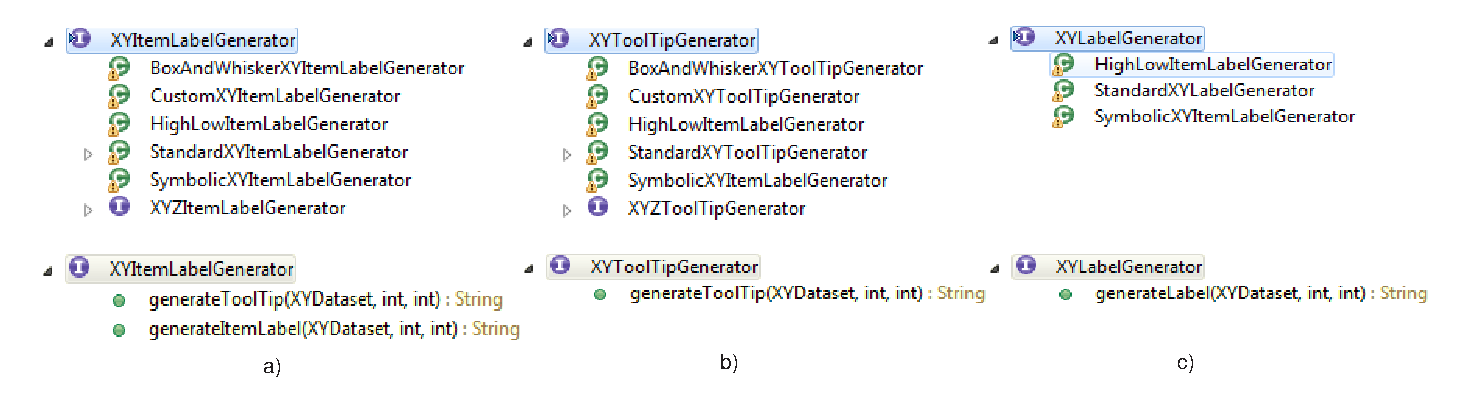
\includegraphics[width=7in]{usage1.eps}}
%\caption{Inheritance and class structure}
%\label{classUsage}
%\end{figure*}
%
%%\begin{figure*}
%%\centerline{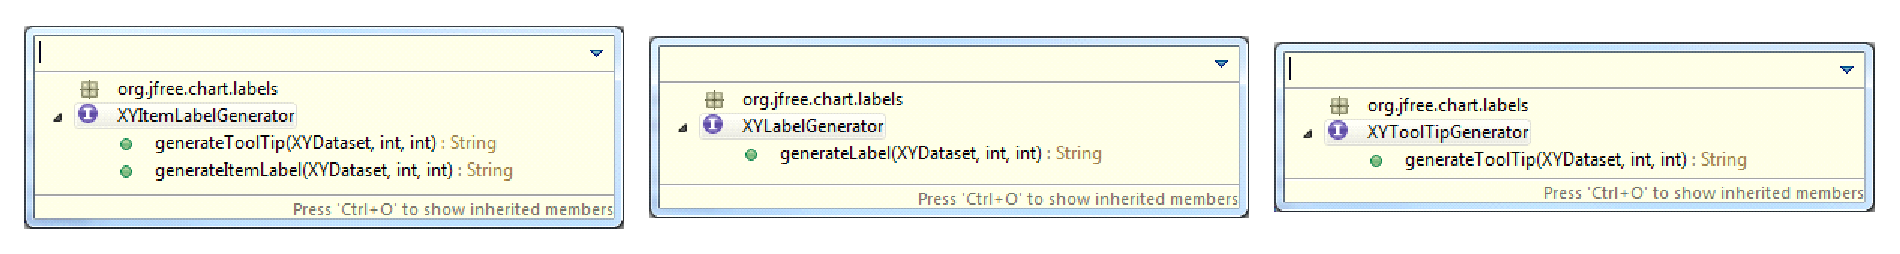
\includegraphics[width=8in]{usage2.eps}}
%%\caption{Class structure}
%%\label{classStruct}
%%\end{figure*}
%
%%\begin{figure*}
%%\centerline{\includegraphics[width=8in]{methodUsage1.eps}}
%%\caption{Method usage}
%%\label{methodUsage1}
%%\end{figure*}
%
%%\begin{figure*}
%%\centerline{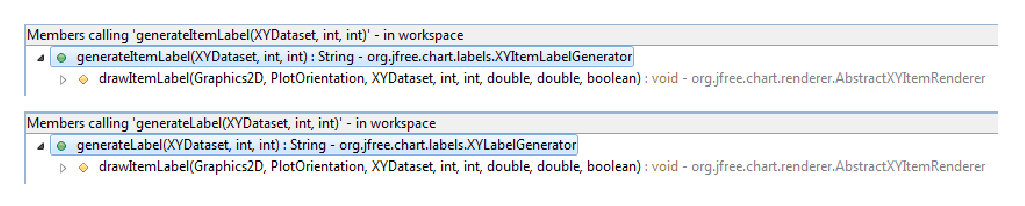
\includegraphics[width=8in]{methodUsage2.eps}}
%%\caption{Method usage}
%%\label{methodUsage2}
%%\end{figure*}
%
%Since graphical charts require textual descriptions, jFreeChart has a
%feature for generating/rendering \emph{labels} and \emph{tooltips} for
%chart items. At version 0.9.17, those two functions of that
%feature are implemented within the interface
%\code{XYItemLabelGenerator} and its descendants, such as
%\code{StandardXYItemLabelGenerator},
%\code{CustomXYItemLabelGenerator}, and
%\code{SymbolicXYItemLabelGenerator}, with two methods
%\code{generateItemLabel} and
%\code{generateToolTip}. Figure~\ref{classUsage}a) illustrates the
%inheritance hierarchy of \code{XYItemLabelGenerator} and its class
%structure.
%
%In version 0.9.17, that feature is realized with two separate class
%hierarchies.
%%those two functions, however, are splitted into two separated class
%%hierarchies.
%The function of \emph{label} generation is implemented in the
%interface \code{XYLabelGenerator} and its descendants, via
%\code{generateLabel} method. The function of \emph{tooltip} generation
%is implemented in the interface \code{XYToolTipGenerator} and its
%descendants, via \code{generateToolTip} method. As shown, during
%evolution, the entities realizing the same feature could be changed in
%their interfaces (e.g. names, locations, parameters) or
%implementations.
%
%Interestingly, the usages of this feature do not change much in the
%system. Moreover, the interactions of the methods/classes of this
%feature with other methods/classes are still quite similar in the
%system. For example, we examined the usages of method
%$A$=\code{XYItemLabelGenerator.generateToolTip} at version 0.9.17 and
%its corresponding method
%$A'$=\code{XYToolTip\-Generator.generateToolTip} at version 0.9.19. We
%saw that $A$ and $A'$ have almost the same set of callers: $A$ has
%sixteen callers and $A'$ has eighteen ones, in which sixteen are the
%same with the ones in $A$ and two are from two newly added
%classes. For two methods \code{XYItemLabelGenerator.generateLabel} and
%\code{XYLabelGenerator.generateLabel}, their callers are exactly the
%same. We also examined the contexts of the calls from those methods to
%other ones in the system and vice versa and found that the contexts of
%such interactions are the same.


%Figure~\ref{methodUsage1}a show the list of callers of
%\code{XYItemLabelGenerator.generateToolTip} within
%jFreeChart. Figure~\ref{methodUsage1}b show the list of callers of
%\code{XYToolTipGenerator.generateToolTip} in the next version. We
%could see that the two lists are the same in two versions. Similarly,
%in Figure~\ref{methodUsage2}, two lists of callers of
%\code{XYItemLabelGenerator.generateLabel} and
%\code{XYLabelGenerator.generateLabel} are also the same.

\subsection{Discussions and Implications}

%Problem statements

As seen in the examples, due to the system's evolution, the program
entities realizing its functionality might be changed in names, source
locations, implementations, or behaviors. A class/method can be {\em
replaced with} or {\em modified into} another one in a new version. If
a developer performs regression testing by running the new version
against existing test cases, (s)he needs to change those existing test
code to fix broken method calls by replacing classes/methods in the
new version. Due to the lack of information, that task could be very
time-consuming. Finding the corresponding entities in the new version
is not straightforward due to the reasons explained earlier.
%Section~\ref{example1sec}.

%%%Moreover, not all existing test cases are required to be adapted.

%If a developer decides to perform regression testing by running the
%new version against existing test cases, (s)he needs to adapt those
%existing test code to use the replacing classes/methods in the new
%version. Due to the lack of documentation, that task is very
%time-consuming with two key challenges. First, finding the
%corresponding entities in the new version is not straightforward due
%to the reasons explained earlier. Second, not all existing test cases
%are required to be adapted.

%If a tester/developer decides to perform regression testing by running
%the new version against existing test cases, (s)he needs to adapt
%those existing test code to use the replacing classes/methods in the
%new version. Due to code evolution and the lack of information, a
%tester often faces two key problems in that task. First, (s)he must
%find by herself/himself those replacements of classes/methods across
%versions. That mapping information is not always available for him/her
%if (s)he is not the author of the source code or if the documentation
%on code changes is not complete. Second, (s)he must go through all
%existing test cases and determine which ones are required to be
%modified in accordance with those replacements. Then, (s)he must
%replace all the references to the old entities with the references to
%the new ones.

This paper addresses the entity tracking problem by introducing
{\tool}, a tool that analyzes two source code versions of a
system and detects the replacements of the classes/methods in which
the entities and their replacements have the same roles in the
system. For example, {\tool} would recommend that
\code{setDragSourceActive} is now replaced by \code{setDragOn}, and
\code{findStackedRangeExtent} is replaced by
\code{getStackedRangeExtent}. {\tool} also identifies the
previous test cases that are required to be repaired in
accordance with those~replacements.

%Therefore, it is desirable to have automated tool support for that
%task during the evolution of the system. A user provides a set of code
%entities of his interest (e.g. classes, methods), and requests the
%tracking tool to detect the replacements/counterparts of those
%entities,   For example, the tool would recommend that the method
%\code{setDragSourceActive} is now replaced by \code{setDragOn}. Such
%recommendation would help him recognize the entities providing the
%functionality of interest in the new version, thus, is useful in
%regression testing tasks.

Developing such an automated tool is challenging because it must take
into account the logical characteristics, such as the dependencies and
interaction of the entities to infer the role similarity in the
system. 
%Tien
%This nature distinguishes the entity tracking problem from that of
%origin analysis, which focuses more on the nature of historical
%existence of entities.
%Tien
%Finding the corresponding entity with the same role via origin
%analysis~\cite{godfrey02,sungkim-wcre05,Kim07} does not always work
%correctly. 
From the view with regard to historical existence, $m$ in jFreeChart
v0.9.20 (Section~\ref{example1sec}) should be mapped to the deprecated
$m$ at v0.9.21. However, {\em repairing existing test cases requires
  $m$ to be mapped to $m'$}. It needs {\em tracking of the entities
  with the same functional role, instead of having the same name or
  location}.

%----------------------------------------------------------------------
The similarity metrics on the entities' names, signatures,
implementation, or callers/callees are applicable. However, an
entity tracking tool cannot solely rely on them because:

1. Entities with the same name might not have the same role, \ie not
  being used in the same way in two versions (see
  Fig.~\ref{example1test}). The names of matched entities might be
  different, \eg due to renaming. Thus, matching entities using only
  the name-based similarity might not always be correct.

2. The callers and/or callees of a method might both be renamed. Thus,
   matching entities solely on the names of their callers/callees
   might be insufficient.

3. The method bodies of matched entities might be quite different
   (Fig.~\ref{drag}). Therefore, using solely code structure-based
   matching would not be sufficient.
%--------------------------------------------------------------------

The functional role of an entity is related to its interaction with
others (\eg how it uses or is used by others). To verify the
interaction/usages of $m$ and $m'$ in jFreeChart v0.9.20 and v0.9.21,
we found that
%all the callers of $m$ were modified to call $m'$.
%Table~\ref{example1} shows that
%Importantly,
they are used in the same set of methods in respective versions. 
%%ASE
%%As seen in Figure~\ref{example1code}, they also call the same
%%ones. 
%%Moreover, the test code is also a method that uses/calls $m$. 
That is, although an entity changes in name or implementation, its
role represented via its \emph{interaction} such as the usage
relations with other entities, is more stable. Thus, the interaction
among code entities can provide useful information for the matching
task. Let us present {\tool}, our novel combination approach of
similarity metrics that also rely on entities' interaction.

%Next, we will present our {\tool} approach.  that provides a novel
% combination of similarity
% measurements based on
% the interactions among entities.


%%%The traditional similarity measurements in original analysis (such as
%%%names, signatures, implementation, callers/callees'
%%%names)~\cite{godfrey02,sungkim-wcre05} are still applicable, however,
%%%an entity tracking tool cannot solely rely on them because:

%%%1. Entities with the same name might not have the same role, i.e. not
%%%  be used in the same way in two versions (see
%%%  Figure~\ref{example1code}). The names of matched entities might be
%%%  different, e.g. due to renaming. Thus, matching entities using only
%%%  the name-based similarity might not always be correct.

%%%2. The callers and/or callees of a method might both be renamed. Thus,
%%%   matching entities solely on the names of their callers/callees
%%%   might be insufficient.

%%%3. The method bodies of matched entities might be quite different
%%%   (Figure~\ref{drag}). Therefore, using solely code structure-based
%%%   matching would not be sufficient.

%In conclusion, the motivating examples suggest the necessity of an
%automated tool for helping developers to tracking entities in evolving
%systems for the purpose of regression testing. Moreover, they suggest
%that such tool cannot solely rely original analysis techniques, but
%should take into account interactions/dependencies among code
%entities. 
